\newpage
\section{手推轮椅主体建模}

\subsection{运动学分析}

	医院和老年机构需要MPW来运送太不适合行走的病人[1]。用户可以通过转动连接在后轮上的手推轮辋来操纵椅子示。
	在该建模中选取对象的机械主体示意如图 \ref{fig:top_view} 所示示。它基本上由两个脚轮和手动后轮组成。在这种建模中已经应用了两轮驱动机器人系统的方法,其中脚轮集中在一起并且假设对系统流施力。 
	$ V_{\rm{CG}} $ 和 $ w_{\rm{CG}} $ 代表质心速度和沿质心转速,$ w_l $ 和 $ w_r $ 分别表示左右车轮的角速度,后手动车轮半径和轮椅宽度由 $ r $ 和 $ L_w $ 表示)。
	下面的矩阵\ref{equ:basic_eq}显示了系统的运动学数学模型:
	
	%%%%%%%%%%%%%%%%%%%%%%%%%%
	\begin{equation}
	\label{equ:basic_eq}
	\begin{bmatrix} \begin{array}{l}{x} \\ {y} \\ {\theta}\end{array} \end{bmatrix}
	=
	r
	\begin{bmatrix}
		\vspace{0.2cm} {\dfrac{\cos \theta}{2}} & {\dfrac{\cos \theta}{2}} \\
		\vspace{0.2cm} {\dfrac{2}{L}} & {\dfrac{\sin \theta}{2}} \\
		{\dfrac{2}{L_w}} & - {\dfrac{2}{L_w}}
	\end{bmatrix}
	\begin{bmatrix} \begin{array}{c}{\omega_r} \\ {\omega_l}\end{array} \end{bmatrix}
	\ ,
	\end{equation}
	%%%%%%%%%%%%%%%%%%%%%%%%%%
	
	\noindent 其中 $ \theta $ 是方位角,$ x $ 和 $ y $ 分别表示系统的几何位置。
	
	以A作为参考点,左右轮的位移课以得到: 
	
	%%%%%%%%%%%%%%%%%%%%%%%%%%
	\begin{equation}
	\label{equ:left_s}
	S_l = h
	-
	\frac{L_w}{2} \sin \theta
	\ ,
	\end{equation}
	%%%%%%%%%%%%%%%%%%%%%%%%%%
	
	%%%%%%%%%%%%%%%%%%%%%%%%%%
	\begin{equation}
	\label{equ:right_s}
	S_r = h
	+
	\frac{L_w}{2} \sin \theta
	\ .
	\end{equation}
	%%%%%%%%%%%%%%%%%%%%%%%%%%
	
	%%%%%%%%%%%%%%%%%
	\begin{figure*}[!h]
		\centering
		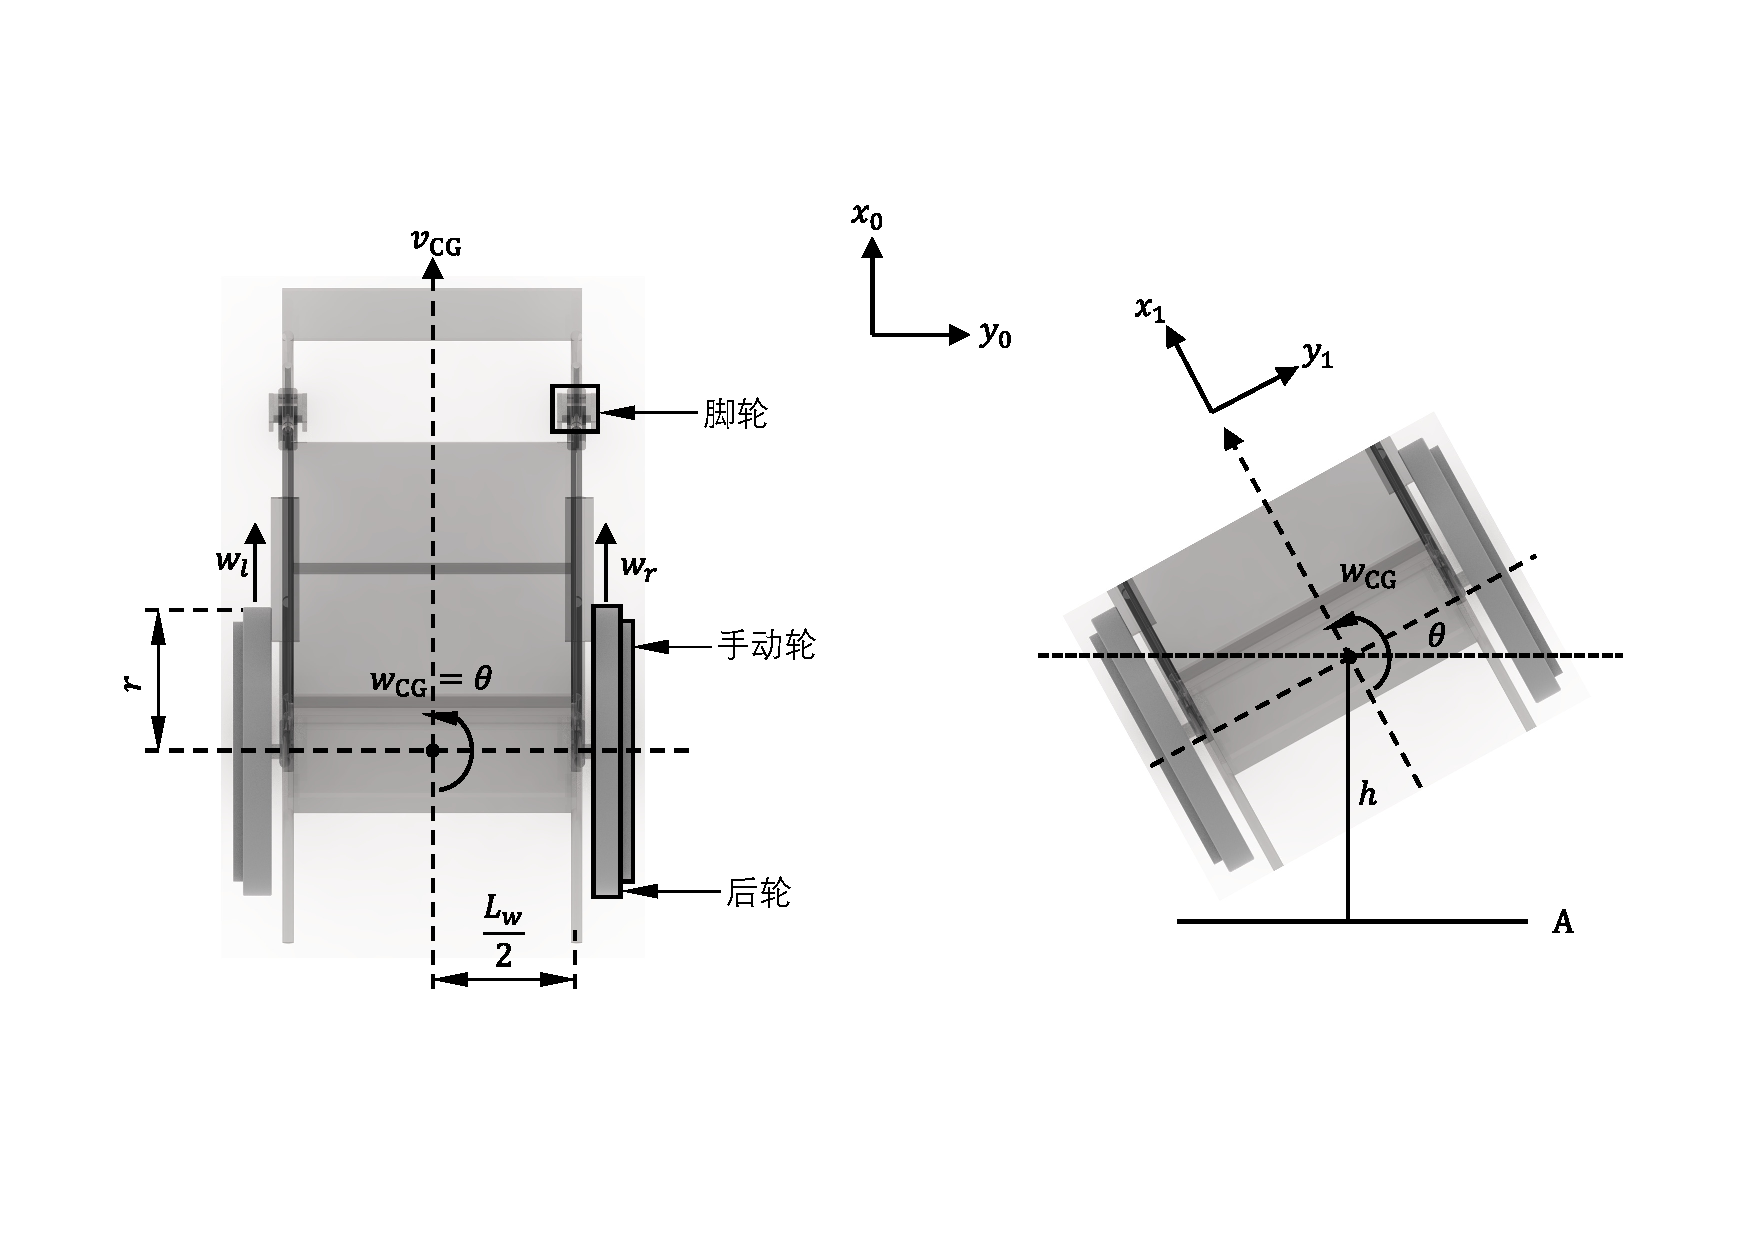
\includegraphics[width=0.96\textwidth]{fig/top_view.pdf}
		\caption{电动轮椅主体俯视示意图。}\label{fig:top_view}
	\end{figure*}
	%%%%%%%%%%%%%%%%%
	
	从键合图出发,广义位移变量定义为流变量的时间积分。因此根据上述方程 \ref{equ:left_s} 和 \ref{equ:right_s},可以获得了所需的流变量方程,将可以通过方程 \ref{equ:left_s} 和 \ref{equ:right_s} 用于构建轮椅主体结构的键合图模型。
	
	%%%%%%%%%%%%%%%%%%%%%%%%%%
	\begin{equation}
	\label{equ:left_w}
	w_{l}
	=
	\dot{S}_{l}
	=
	\dot{h}
	-
	\dot{\theta} \frac{L_w}{2} \cos \theta
	\ ,
	\end{equation}
	%%%%%%%%%%%%%%%%%%%%%%%%%%
	
	%%%%%%%%%%%%%%%%%%%%%%%%%%
	\begin{equation}
	\label{equ:right_w}
	w_{r}
	=
	\dot{S}_{r}
	=
	\dot{h}
	+
	\dot{\theta} \frac{L_w}{2} \cos \theta
	\ .
	\end{equation}
	%%%%%%%%%%%%%%%%%%%%%%%%%%
	
	根据图\ref{fig:top_view},我们用 $ V_{\rm{CG}} $ 和 $ w_{\rm{CG}} $ 分别表示质心速度和角速度。
	
	轮椅上的平均受力等于通过系统总质量与 $ V_{\rm{CG}} $ 相关的线性动量的变化率之比,如下所示:
	
	%%%%%%%%%%%%%%%%%%%%%%%%%%
	\begin{equation}
	\label{equ:V_CG}
	V_{\rm{CG}}
	=
	\frac{P_{\rm{CG}}}{M_t}
	\ .
	\end{equation}
	%%%%%%%%%%%%%%%%%%%%%%%%%%
	
	质心处的平均扭矩等于通过系统惯性矩与 $ w_{\rm{CG}} $ 相关的角动量的变化率之比,如下所示:
	
	%%%%%%%%%%%%%%%%%%%%%%%%%%
	\begin{equation}
	\label{equ:w_CG}
	w_{\rm{CG}}
	=
	\frac{P_{\theta}}{J}
	\ .
	\end{equation}
	%%%%%%%%%%%%%%%%%%%%%%%%%%

\subsection{各部分键合图导出}

	正在完成!

\subsection{手推轮椅部分键合图}

	在该部分中,我们假设手推动力作为输入源。
	{\color{blue} 图xxx}中描绘的轮椅主体键合图模型由上述组件构成。轮椅机械主体的因果关系根据主体系统的约束进行调整。由后轮上的手推动扭矩产生的能量传递到系统结构,如图键合半箭头所示。
	所有外部扭矩和转动惯量都连接到1结,L和R代表系统的左侧和右侧。 这些交汇点的本构方程,其中整个系统的质量和惯性矩运用了牛顿第二定律。
	理想的换能器TF表示通过后轮半径的能量转换。

